\title[概率论]{第九讲:常见的离散型随机变量}
\institute[东南大学数学学院]{\large \textrm{Email: xzhangseu@seu.edu.cn} \\ \quad  \\
	\large 东南大学 \quad 数学学院 \\
	\vspace{0.3cm}
	%  \trc{公共邮箱: \textrm{zy.prob@qq.com}\\
	%    \hspace{-1.7cm}  密 \qquad 码: \textrm{seu!prob}}
}
\date{}


{ \setbeamertemplate{footline}{}
	\begin{frame}
		\titlepage
	\end{frame}
}
% \begin{CJK*}{GBK}{song}

%   \title{简单随机抽样}
%   \author{林语堂}
%   \institute{University}
%   \date{2009-03-31}
%   \date{}
%   \begin{frame}
%     \titlepage
%   \end{frame}

%   \begin{frame}
%     \frametitle{第二章:简单随机抽样}
%     \tableofcontents
%   %     You might wish to add the option[pausesections]
%   \end{frame}

%   \AtBeginSubsection[]{
%   \begin{frame}<beamer>
%     \frametitle{Outline}
%     \tableofcontents[currentsection,currentsubsection]
%   \end{frame}
% }
%   定义目录页



% \begin{frame}[plain]
%   \frametitle{目录}
%   \setcounter{tocdepth}{2}
%   \tableofcontents
% \end{frame}
\addtocounter{framenumber}{-3}  % 目录页不计算页码
%\section{随机变量}
\subsection{伯努利试验及其离散型分布}
\begin{frame}
	\frametitle{伯努利实验}
	\begin{itemize}[<+-|alert@+>]
		\item 只有两种可能结果的试验称为伯努利试验;例如抽检产品,可能是合格品,也可能是次品;掷两颗骰子,可能得到同点,也可能得到不同点,等等都是伯努利试验.
		\item 伯努利试验的样本空间 $\Omega$ 并不一定只含有两个样本点,有时只是把我们所关心的一部分样本点归结为一种结果 $A$, 同时把其余的样本点的集合看作另一种结果 $\bar{A}$;
		\item 在上述掷骰子的试验中,样本空间 $\Omega$ 共含有 36 个样本点,如果我们只关心同点是否发生,就可以把其中的 6 个样本点组成的事件 $A:=\{(i,i):i=1,\cdots, 6\}$ 视为一种结果,而其余的 30 个样本点组成另一结果 $\bar{A}:=\{\mbox{不同点}\}$;
		\item 此外我们不再关心由 $\Omega$ 的其他非空子集组成的事件,于是对于伯努利试验而言,事件 $\sigma$ 代数应取为 $\mathcal{F}=\{\emptyset, A, \bar{A}, \Omega\}$;
		\item 通常把结果 $A$ 称作 "成功", 而把 $\bar{A}$ 称作 "失败";
		\item 再取定成功失败的概率 $p=P (A), q=P (\bar{A})$ ($p>0,q>0$ 且 $p+q=1$), 则建立了一次伯努利试验的概率空间 $(\Omega,\mathcal{F},P)$.
	\end{itemize}
\end{frame}
\begin{frame}
	\begin{itemize}[<+-|alert@+>]
		\item 在概率论的理论与应用中,经常以一系列独立重复的伯努利试验作为概率模型;
		\item 所谓重复,粗略的说即各次试验的概率空间都是上述的 $(\Omega,\mathcal{F},P)$;
		\item 而 $n$ 个试验的独立性则是指各次试验的结果互不影响,即对于第 $i$ 次试验的任何结果 $E_i (i=1,\cdots, n)$ 均有
		      \begin{eqnarray*}
			      P(E_1E_2\cdots E_n)=P(E_1)P(E_2)\cdots P(E_n)
		      \end{eqnarray*}
		\item 将一次伯努利试验独立重复 $n$ 次,称作 $n$ 重伯努利试验;
		\item 将一次伯努利试验独立地重复下去所得到的一系列试验,称为可列重伯努利试验.
	\end{itemize}
\end{frame}

\begin{frame}
	\frametitle{二项分布:$n$ 重伯努利试验中成功的次数 $X$}
	\begin{itemize}[<+-|alert@+>]
		\item $X$:$n$ 重伯努利试验中成功 (事件 $A$ 发生) 的次数;
		\item $X$ 的所有可能取值为: $0, 1, \cdots, n$;
		\item 下面我们考虑 $X$ 的分布列
		      \begin{itemize}
			      \item $n$ 重伯努利试验的样本空间: $\Omega:=\{\omega=(\omega_1,\cdots,\omega_n):\omega_i\mbox{或者为} A\mbox{或者为}\bar{A}\}$
			      \item 样本空间样本点的个数为 $2^n$ 个;
			      \item $\{X=k\}=\{\omega=(\omega_1,\cdots,\omega_n):\omega_1,\cdots,\omega_n\mbox{中有} k\mbox{个} A\}$, 共包含 $C_n^k$ 个样本点;
			      \item 若任给样本点 $\omega=(\omega_1,\cdots,\omega_n)\in \{X=k\}$, 则意味着 $\omega_1,\cdots,\omega_n$ 中有 $k$ 个 $A$, $n-k$ 个 $\bar{A}$, 故由独立性可知
			            \begin{eqnarray*}
				            P(\omega)=p^k(1-p)^{n-k}
			            \end{eqnarray*}
			      \item 而事件 $\{X=k\}$ 中共有 $C_n^k$ 个类似的 $\omega$, 故
			            \begin{eqnarray*}
				            P(X=k)=C_n^kp^k(1-p)^{n-k}:=b(k;n,p), k=0,1,\cdots, n
			            \end{eqnarray*}
			            这个分布常称为二项分布,记为 $X\sim B (n,p)$.
			      \item 容易验证,$\sum_{k=0}^nC_n^kp^k (1-p)^{n-k}=(p+1-p)^n=1$
		      \end{itemize}
	\end{itemize}

\end{frame}
\begin{frame}
	\frametitle{两点分布}
	\begin{itemize}
		\item $n=1$ 时的二项分布 $B (1,p)$ 称为二点分布,或 $0-1$ 分布,或称伯努利分布,其分布列为
		      \begin{eqnarray*}
			      P(X=k)=p^k(1-p)^{1-k}, k=0, 1
		      \end{eqnarray*}
		      或记为
		      \begin{eqnarray*}
			      \left(\begin{array}{cc}
				      0,   & 1  \\
				      1-p, & p
			      \end{array}\right)
		      \end{eqnarray*}
		\item $B (1,p)$ 主要用于描述一次伯努利试验中成功的次数 (0 或 1);
		\item 若记 $X_i$ 表示第 $i$ 次伯努利试验中成功的次数,则 $X_i$ 相互独立且有
		      \begin{eqnarray*}
			      X=X_1+X_2+\cdots X_n
		      \end{eqnarray*}
		      即二项分布随机变量可写为 $n$ 个独立同为两点分布随机变量的和.
	\end{itemize}
\end{frame}
\begin{frame}
	\frametitle{二项分布的性质}
	\begin{itemize}[<+-|alert@+>]
		\item 对 $k\ge 1$, 考虑比值
		      \begin{eqnarray*}
			      \dfrac{b(k;n,p)}{b(k-1;n,p)}&=&\pause \dfrac{C_n^kp^k(1-p)^{n-k}}{C_n^{k-1}p^{k-1}(1-p)^{n-k+1}}=\pause \dfrac{(n-k+1)p}{k(1-p)}\\
			      &=&\pause \dfrac{k(1-p)+(n+1)p-k}{k(1-p)}=\pause 1+\dfrac{(n+1)p-k}{k(1-p)}
		      \end{eqnarray*}
		\item 当 $(n+1) p>k$ 时,$b (k;n,p)>b (k-1;n,p)$;
		\item 当 $(n+1) p<k$ 时,$b (k;n,p)<b (k-1;n,p)$;
		\item 从而,对于固定的 $n,p$,$\{X=k\}$ 的概率 $b (k;n,p)$ 先随 $k$ 增大而增大,再随 $k$ 增大而减小,故必有最大值:
		      \begin{itemize}
			      \item 如果 $m:=(n+1) p$ 为整数,则 $b (m;n,p)=b (m-1;n,p)$ 同为 $b (k;n,p)$ 的最大值
			      \item 如果 $(n+1) p$ 不为整数,则 $b (k;n,p)$ 在 $m=[(n+1) p]$ 处取到最大值 (此处 $[a]$ 表示不超过 $a$ 的最大整数)
		      \end{itemize}
		\item 我们称使得 $b (k;n,p)$ 取得最大值的 $m$ 为二项分布随机变量的最可能值,或称为 $n$ 重伯努利试验中最可能的成功次数.
	\end{itemize}
\end{frame}


\begin{frame}{二项分布的性质}
	\begin{thm}\label{338} 设 $X\sim B (n,p)$, 且 $q=1-p$(通常用 $q$ 表示伯努利试验失败的概率), 则有 $n-X\sim B (n,q)$.
	\end{thm}

	\pause
	% \begin{jieda}
	\begin{itemize}[<+-|alert@+>]
		\item 借用二项分布的直观定义:将 $X$ 为 $n$ 次独立伯努利试验成功的次数,则 $n-X$ 为这些试验中失败的次数.
		\item 互相交换成功与失败的角色,可知 $n-X\sim B (n,q)$.
		\item 也可从分布列 (概率质量函数) 的角度出发得到
		      $n-X\sim B(n,q).$
		\item 令 $Y=n-X$, 则 $Y$ 的分布列 (概率质量函数) 为 \pause
		      \begin{equation*}
			      \begin{aligned}
				      P(Y=k)= & P(n-X=k)=P(X=n-k)                                                           \\
				      =       & \left(\begin{matrix}
						                      n   \\
						                      n-k \\
					                      \end{matrix}\right)p^{n-k}q^{k}=\left(\begin{matrix}
						                                                            n \\
						                                                            k \\
					                                                            \end{matrix}\right)q^kp^{n-k},
			      \end{aligned}
		      \end{equation*}
	\end{itemize}
	% \end{jieda}
\end{frame}

\begin{frame}{二项分布的性质}

	\begin{thm} 设 $X\sim B (n,p)$, 其中 $n$ 为偶数,$p=1/2$, 则 $X$ 的分布关于 $n/2$ 对称,即对任意的非负整数 $j$, 均有
		$$P(X=\frac{n}{2}+j)=P(X=\frac{n}{2}-j).$$
	\end{thm}
	\pause
	%\vspace{0.2cm}

	\begin{jieda} 由定理 \ref{338} 可知,$n-X$ 同样服从 $B (n,1/2)$. \pause 因此对任意非负整数 $k$ 均有
		$$P(X=k)=P(n-X=k)=P(X=n-k).$$
		\pause
		令 $k=n/2+j$, 即可得证. % 得推论 \ref{338} 的结果。该推论也解释了为什么图 3.6 中 $Bin (10,1/2)$ 是关于 5 对称的.
	\end{jieda}

	%\begin{exam}({\tc 掷硬币续}) 回顾例 \ref{312}, 现在已经知道 $X\sim Bin (2,1/2),Y~\sim Bin (2,1/2)$ 和 $I\sim Bern (1/2)$. 由定理 \ref{337} 可知,$X$ 和 $Y=2-X$ 具有相同的分布。再根据推论 \ref{338}, 得到 $X$ 的分布 (以及 $Y$ 的分布) 是关于 1 对称的.
	%\end{exam}
\end{frame}






\begin{frame}
	\vspace{0.4cm}
	\begin{exam}
		设每台自动机床在运行过程中需要维修的概率均为 $p=0.01$, 并且各机床是否需要维修相互独立。如果:
		\begin{enumerate}
			\item 每名维修工人负责看管 20 台机床;
			\item 3 名维修工人负责看管 80 台机床;
		\end{enumerate}
		求机床不能及维修的概率.
	\end{exam}

	\pause \jieda 1. 这是 $n=20$ 重伯努利试验,参数 $p=0.01$, 故需要维修的机床数 $X$ 服从 $B (20,0.01)$ 分布。故不能及时维修的概率为 \pause
	\begin{eqnarray*}
		P(X>1)&=&\pause 1-P(X\le 1)=\pause 1-P(X=0)-P(X=1)\\
		&=&\pause 1-C_{20}^00.01^0(1-0.01)^{20}-C_{20}^10.01(1-0.01)^{20-1}\approx 0.0169
	\end{eqnarray*}
	\pause 2. 此时需要维修的机床数 $X$ 服从 $B (80,0.01)$ 分布,类似可得不能及时维修的概率为
	\begin{eqnarray*}
		P(X>3)=1-\sum_{k=0}^3b(k;80,0.01)\approx 0.0087
	\end{eqnarray*}

\end{frame}

\begin{frame}
	\frametitle{小概率事件终将发生}
	\begin{exam}
		在可列重伯努利试验中,求事件 $E:=\{\mbox{试验终将成功}\}$ 的概率.
	\end{exam}
	\pause

	\jieda 考虑所求概率事件的反面即 $\overline{E}:=\{\mbox{试验永不成功}\}$.\pause 若我们记
	\begin{eqnarray*}
		F_n:=\{\mbox{前} n\mbox{次试验均失败}\},
	\end{eqnarray*}
	\pause
	则易知,$\{F_n\}$ 为单调下降事件序列,且
	\begin{eqnarray*}
		\lim_{n\rightarrow \infty}F_n=\pause \cap_{n=1}^\infty F_n=\pause \overline{E}
	\end{eqnarray*}
	\pause 从而
	\begin{eqnarray*}
		P(\overline{E})=\pause P(\lim_{n\rightarrow\infty}F_n)=\pause \lim_{n\rightarrow\infty }P(F_n)=\pause \lim_{n\rightarrow\infty }C_n^0p^0(1-p)^n=\pause 0
	\end{eqnarray*}
	\pause 故
	\begin{eqnarray*}
		P(E)=1-P(\overline{E})=1-0=1
	\end{eqnarray*}
	\pause 无论成功的概率有多小,但是试验最终成功的概率为 1, 也就是说小概率事件终将发生的概率为 1.
\end{frame}

%   \title[概率论]{第十一讲:常见的离散型随机变量 (II)}
%   \author[张鑫 {\rm Email: x.zhang.seu@foxmail.com} ]{\large 张 鑫}
%   \institute[东南大学数学学院]{\large \textrm{Email: x.zhang.seu@foxmail.com} \\ \quad  \\
%   	\large 东南大学 \quad 数学学院 \\
%   	\vspace{0.3cm}
%   	%  \trc{公共邮箱: \textrm{zy.prob@qq.com}\\
%   		%    \hspace{-1.7cm}  密 \qquad 码: \textrm{seu!prob}}
%   }
%   \date{}



%   	{ \setbeamertemplate{footline}{}
%   		\begin{frame}
%   			\titlepage
%   		\end{frame}
%   	}

%   	% \begin{frame}[plain]
%   		%   \frametitle{目录}
%   		%   \setcounter{tocdepth}{2}
%   		%   \tableofcontents
%   		% \end{frame}
%   	\addtocounter{framenumber}{-3}  % 目录页不计算页码
%   	\section{随机变量}
%   	\subsection{伯努利试验及其离散型分布}

\begin{frame}
	\frametitle{几何分布:可列重伯努利试验中首次成功的等待时间 $X$}
	\begin{itemize}[<+-|alert@+>]
		\item 记 $X$ 为可列重伯努利试验中首次成功的等待时间即首次成功所需要试验的次数;
		\item $\{X=k\}=\{\underbrace{\overline{A}\cdots \overline{A}}_{k-1\mbox{个}} A\}$, 故
		      \begin{eqnarray*}
			      P(X=k)=(1-p)^{k-1}p:=g(k;p), k=1,\cdots,
		      \end{eqnarray*}
		      这个分布常称为几何分布,记为 $X\sim G (p)$.
	\end{itemize}
\end{frame}
\begin{frame}
	\frametitle{几何分布的性质}
	\begin{thm}
		取值自然数的随机变量 $X$ 为几何分布当且仅当 $X$ 有无记忆性:
		\begin{eqnarray}\label{eq:memory}
			P (X>m+n|X>m)=P (X>n), \mbox{对任意的} m,n \ge 1.
		\end{eqnarray}
	\end{thm}
	\zheng 若 $X$ 为几何分布,则
	\begin{eqnarray*}
		P(X>m+n|X>m)=\pause \dfrac{P(X>m+n,X>m)}{P(X>m)}=\pause \dfrac{P(X>m+n)}{P(X>m)}
	\end{eqnarray*}
	\pause 而
	\begin{eqnarray*}
		P(X>n)=\pause \sum_{k=n+1}^\infty (1-p)^{k-1}p=\pause \dfrac{(1-p)^{n}p}{1-(1-p)}=\pause (1-p)^n
	\end{eqnarray*}
	\pause 故
	\begin{eqnarray*}
		P(X>m+n|X>m)=\dfrac{(1-p)^{m+n}}{(1-p)^m}=(1-p)^n=P(X>n)
	\end{eqnarray*}

\end{frame}

\begin{frame}
	\vspace{0.5cm}
	若 $X$ 具有无记忆性,则由~\eqref{eq:memory} 知
	\pause \begin{eqnarray*}
		Q_n:=P (X>n)>0, \quad \mbox{对任意的} n\ge 1
	\end{eqnarray*}
	\pause 并且有
	\begin{eqnarray*}
		Q_{m+n}=P(X>m+n)=\pause P(X>m)P(X>m+n|X>m)=\pause Q_mQ_n
	\end{eqnarray*}
	\pause 从而 \vspace{-0.7cm}
	\begin{eqnarray*}
		Q_m=Q_1^m
	\end{eqnarray*}
	\pause 注意到 $Q_1\in (0,1)$, 事实上,
	\begin{itemize}[<+-|alert@+>]
		\item $Q_1=P (X>1)>0$ 显然;
		\item  若 $Q_1=1$, 则对一切的 $m$ 均有 $Q_m=P (X>m)=1$, 这与 $X$ 取自然数矛盾,故 $Q_1\in (0,1)$.
	\end{itemize}
	\pause 故取 $p=1-Q_1\in (0,1)$, 且对任意的 $k\ge 1$ 有
	\begin{eqnarray*}
		P(X=k)&=&\pause P(X>k-1)-P(X>k)=\pause Q_{k-1}-Q_k\\
		&=&\pause (1-p)^{k-1}-(1-p)^k=\pause (1-p)^{k-1}p
	\end{eqnarray*}

\end{frame}

\begin{frame}
	\frametitle{无记忆性}
	\begin{eqnarray*}
		P(X>m+n|X>m)=P(X>n)
	\end{eqnarray*}
	\begin{itemize}[<+-|alert@+>]
		\item 上述的无记忆性表明:已知试验了 $m$ 次未获得成功,再加做 $n$ 次试验仍不成功的概率,等于从开始算起做 $n$ 次试验都不成成功的概率.
		\item 换句话放,已做过的 $m$ 次失败的试验被忘记了;
		\item 产生几何分布的这种无记忆性的根本原因在于,我们进行的是独立重复试验,这是不学习,不总结经验的试验,已经做过的试验当然不会留下记忆.
	\end{itemize}
\end{frame}

\begin{frame}
	\vspace{0.3cm}
	\begin{exam}
		10 把外形相同的钥匙中只有一把能打开门。现一一试开,试对每次试毕放回与不放回两种情形,分别求事件 $E:=\{\mbox{至多试} 3\mbox{次能打开门}\}$ 的概率.
	\end{exam}

	\pause
	\jieda 1. 放回情形是独立重复试验,属伯努利概型。以 $X$ 表示首次打开门的等待时间,则 $X$ 服从几何分布 $G (0.1)$. 故所求概率为
	\begin{eqnarray*}
		P(E)=P(X\le 3)=\sum_{k=1}^3(1-0.1)^{k-1}0.1=0.271
	\end{eqnarray*}
	\pause
	2. 不放回情形不再是独立重复试验,适用于古典概型。样本点总数 $n (\Omega)=C_{10}^3$, 而 $n (\overline{E})=C_9^3$. 故
	\begin{eqnarray*}
		P(E)=1-P(\overline{E})=1-\dfrac{C_9^3}{C_{10}^3}=0.3
	\end{eqnarray*}
	\pause 或令 $A_i:=\{\mbox{第} i\mbox{次取到能开门的钥匙}\}$, 则 $A_1,A_2,A_3$ 互不相容,由可加性及抽签的公平性可得
	\begin{eqnarray*}
		P(E)=P(\cup_{i=1}^3A_i)=\sum_{i=1}^3P(A_i)=0.3
	\end{eqnarray*}

\end{frame}
\begin{frame}
	\frametitle{帕斯卡 (Pascal) 分布:第 $r$ 次成功的等待时间}
	\begin{itemize}[<+-|alert@+>]
		\item 记 $X_r$ 为可列重伯努利试验中第 $r$ 次成功的等待时间即第 $r$ 次成功所需要试验的次数;
		\item 易见 $X$ 的所有可能取值为 $k=r, r+1,\cdots, $ 并且有
		      \begin{eqnarray*}
			      \{X_r=k\}&=&\{\mbox{前} k-1\mbox{次试验恰有} r-1\mbox{次成功且第} k\mbox{次成功}\}\\
			      \pause
			      P (X_r=k)&=&\pause P (\mbox{前} k-1\mbox{次试验恰有} r-1\mbox{次成功}) P (\mbox{第} k\mbox{次成功})\\
			      &=&\pause C_{k-1}^{r-1}p^{r-1}(1-p)^{k-1-(r-1)}p\\
			      &=&\pause C_{k-1}^{r-1}p^r(1-p)^{k-r}:=f(k;r,p), \quad k=r, r+1,\cdots
		      \end{eqnarray*}
		      \pause 这个分布常称为帕斯卡 (Pascal) 分布或负二项分布.
		\item $f (k;r,p), k=r,r+1,\cdots,$ 可以成为离散型分布的密度,事实上: $f (k;r,p)>0$ 显然,其和
		     {\small \begin{eqnarray*}
			      \sum_{k=r}^\infty f(k;r,p)&=&\pause  \sum_{k=r}^\infty C_{k-1}^{r-1}p^r(1-p)^{k-r}\xlongequal[q=1-p]{k-r=i}\pause \sum_{i=0}^\infty C_{r+i-1}^{r-1}p^rq^{r+i-r}\\
			      &=&\pause \sum_{i=0}^\infty C_{r+i-1}^ip^rq^i=\pause \sum_{i=0}^\infty C_{-r}^ip^r(-q)^i=\pause p^r(1-q)^{-r}=1 \end{eqnarray*}
		      }
	\end{itemize}
\end{frame}
\begin{frame}
	\frametitle{帕斯卡分布的性质}
	\begin{itemize}[<+-|alert@+>]
		\item 若帕斯卡分布中的 $r=1$, 则此时的帕斯卡分布即为几何分布;
		\item 如果记 $$\tau_1=X_1, \quad \tau_n=X_n-X_{n-1}, \quad n>1, $$ 则随机变量 $\tau_n$ 是第 $n-1$ 次成功到第 $n$ 次成功的间隔时间。显然有
		      \begin{eqnarray*}
			      X_r=\tau_1+\tau_2+\cdots+\tau_r
		      \end{eqnarray*}
		\item 以后我们会看到: $\tau_1,\cdots, \tau_r$ 是 $r$ 个相互独立的随机变量且每个 $\tau_k$ 均服从几何分布.
	\end{itemize}
\end{frame}

\begin{frame}
	\begin{exam}
		某人口袋中有两盒火柴,开始时每盒各装 $n$ 根。每次他从口袋中任取一盒使用其中的一根火柴。求此人掏出一盒发现已空,而另一盒尚余 $r$ 根的概率.
	\end{exam}

	\pause
	\jieda 记
	\begin{eqnarray*}
		E=\{\mbox{掏出甲盒已空而乙盒尚余} r\mbox{根}\}
	\end{eqnarray*}
	\pause 则由对称性可知所求概率为 $2P (E)$. \pause 若我们以取出甲盒为 "成功", 这便是一个成功率 $p=1/2$ 的独立重复伯努利试验.
	\pause 而
	\begin{eqnarray*}
		E=\{\mbox{第} n+1\mbox{次成功发生在第} 2n-r+1\mbox{次试验}\}
	\end{eqnarray*}
	\pause 故所求概率为
	\begin{eqnarray*}
		2P(E)&=&\pause 2f(2n-r+1;n+1,1/2)=\pause 2C_{2n-r}^n(\dfrac{1}{2})^{n+1}(\dfrac{1}{2})^{2n-r-n}\\
		&=&\pause C_{2n-r}^n2^{r-2n}
	\end{eqnarray*}

\end{frame}


\begin{frame}
	\frametitle{分赌注问题}
	\begin{exam}
		1654 年,当时的职业赌徙 DeMere 爵士向法国的大数学家 Pascal 提出如下问题:甲乙两人各下赌注 $m$ 元,商定先胜三局者取得全部赌金。假定在每一局中二人获胜的机会相等,且各局胜负相互独立。如果当甲胜一局而乙胜零局时赌博被迫中止,问赌注如何分?
	\end{exam}
	\pause
	\begin{itemize}[<+-|alert@+>]
		\item 为解决这个问题,Pascal 与当时声望很高的数学家 Fermat 建立了通信联系。他们进行了卓有成效的讨论,不仅完满的回答了分赌注问题,而且为解决其他概率问题建立起了框架,极大的促进了概率论的建立与发展;
		\item Pascal 令人信服的指出,赌金的分法应当取决于若赌博能继续进行下去甲乙各自获胜的概率,这个概率即为在 $p=0.5$ 的可列重伯努利试验中 2 次成功发生在 3 次失败之前的概率;
		\item 更一般的,下面我们求一下 $n$ 次成功发生在 $m$ 次失败之前的概率.
	\end{itemize}
\end{frame}

\begin{frame}
	\begin{exam}
		在可列重伯努利试验中,求下面事件的概率: $$E=\{n\mbox{次成功发生在} m\mbox{次失败之前}\}$$
	\end{exam}
	\pause \jieda 记 $F_k=\{\mbox{第} n\mbox{次成功发生在第} k\mbox{次试验}\}$, 则
	\begin{eqnarray*}
		E=\cup_{k=n}^{n+m-1}F_k
	\end{eqnarray*}
	\pause 从而由 $F_k$ 的互不相容性可得
	\begin{eqnarray*}
		P(E)=\sum_{k=n}^{n+m-1}P(F_k)=\sum_{k=n}^{n+m-1}C_{k-1}^{n-1}p^n(1-p)^{k-n}
	\end{eqnarray*}
	\pause 利用上面的公式可计算 $n=2,m=3, p=1/2$ 时,其相应的概率为
	\begin{eqnarray*}
		P (\mbox{甲胜})=P (E)\xlongequal{n=2,m=3,p=1/2}\dfrac{11}{16}
	\end{eqnarray*}
	故赌注应以 $11:5$ 的比例分配给甲乙两人.
\end{frame}
\subsection{泊松分布}
\begin{frame}
	\begin{columns}
		\column{4cm}
		\begin{figure}[htbp]\nonumber
			\centering
			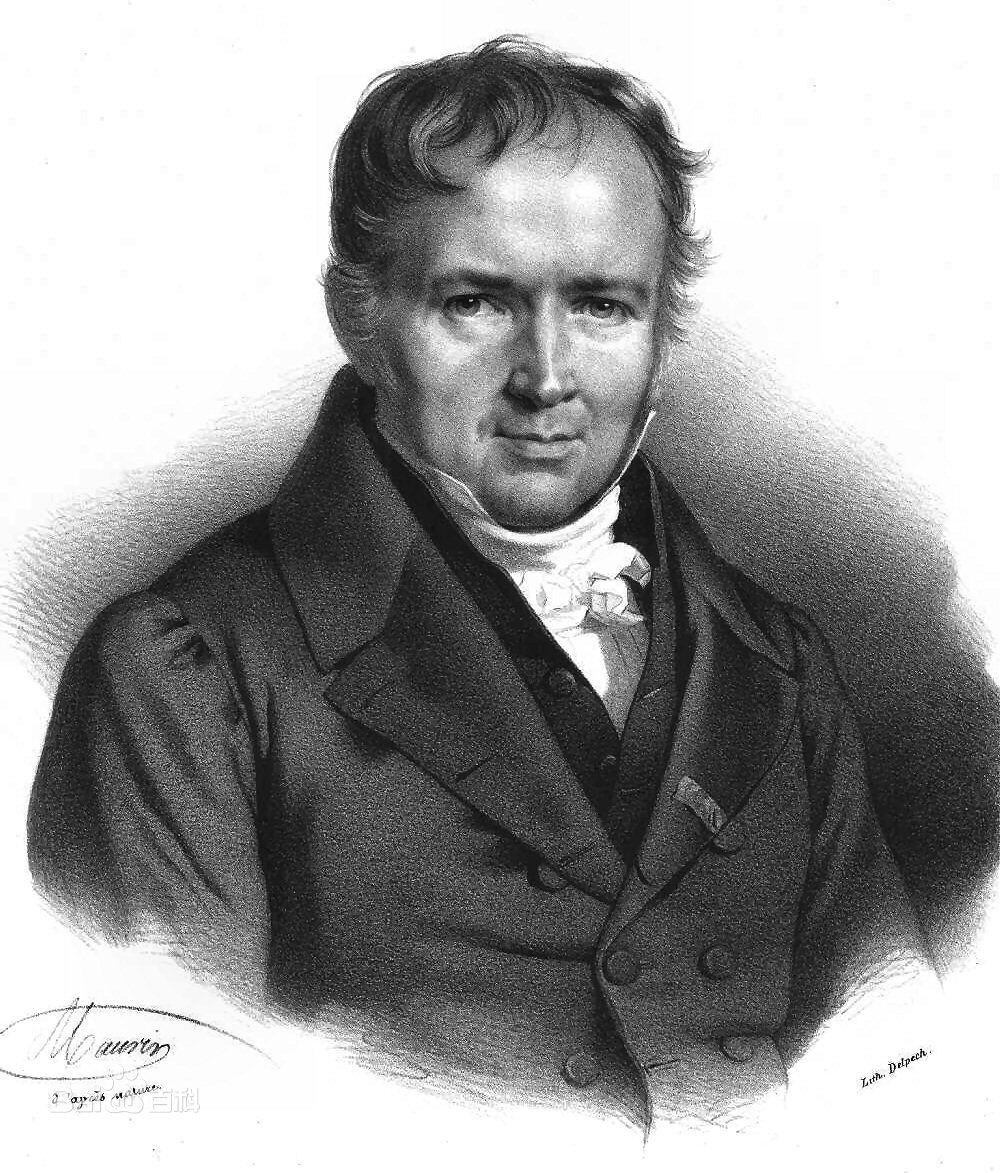
\includegraphics[width=4cm]{p1.jpg}
			\caption{泊松}
		\end{figure}
		\pause
		\column{6cm}
		\begin{itemize}[<+-|alert@+>]
			\item 西莫恩・德尼・泊松:法国数学家、几何学家和物理学家;
			      % \item 1781 年 6 月 21 日生于法国卢瓦雷省的皮蒂维耶,1840 年 4 月 25 日卒于法国索镇;
			\item 泊松的科学生涯开始于研究微分方程及其在摆的运动和声学理论中的应用;
			\item 对积分理论、行星运动理论、热物理、电磁理论、位势理论和概率论都有重要贡献;
			\item 19 世纪概率统计领域里的卓越人物,改进了概率论的运用方法,特别是用于统计方面的方法,建立了描述随机现象的一种概率分布──泊松分布;
			\item 推广了 “大数定律”,并导出了在概率论与数理方程中有重要应用的泊松积分。
		\end{itemize}


	\end{columns}
\end{frame}

\begin{frame}
	\frametitle{泊松 (Poisson) 分布}
	\begin{itemize}[<+-|alert@+>]
		\item Poisson 分布是概率论中一种重要的离散型分布,它在理论与实践中都有广泛的应用,常与单位时间 (面积) 内上的计数过程相联系;
		      \begin{itemize}
			      \item 一天内到达某商场的顾客数;
			      \item 单位时间内,电路受外界电磁波的冲击次数;
			      \item 一定时期内,某放射性物质放射出来的粒子数等
		      \end{itemize}
		\item 在二项分布中,当参数 $n$ 较大时,计算二项概率 $b (k;n,p)$ 会非常麻烦.
	\end{itemize}
	\pause  \begin{thm}
		设有一列二项分布 $\{b (k;n,p_n)\}$, 若其参数列 $p_n$ 满足
		\begin{eqnarray*}
			\lim_{n\rightarrow \infty}np_n=\lambda>0,
		\end{eqnarray*}
		则对任何非负整数 $k$ 有
		\begin{eqnarray*}
			\lim_{n\rightarrow \infty}b(k;n,p_n)=\dfrac{\lambda^k}{k!}e^{-\lambda}.
		\end{eqnarray*}
	\end{thm}
\end{frame}
\begin{frame}

	\vspace{0.4cm}
	\zheng 记 $\lambda_n:=np_n$, 则
	\begin{eqnarray*}
		b(k;n,p_n)&=&\pause C_n^kp_n^k(1-p_n)^{n-k}=\pause \dfrac{n!}{k!(n-k)!}(\dfrac{\lambda_n}{n})^k(1-\dfrac{\lambda_n}{n})^{n-k}\\
		&=&\pause \dfrac{\lambda_n^k}{k!}(1-\dfrac{1}{n})(1-\dfrac{2}{n})\cdots(1-\dfrac{k-1}{n})(1-\dfrac{\lambda_n}{n})^{n-k}
	\end{eqnarray*}
	\pause 注意到
	\begin{eqnarray*}
		&&\pause \lim_{n\rightarrow\infty}\lambda_n^k=\lambda^k, \\
		&&\pause \lim_{n\rightarrow\infty}(1-\dfrac{1}{n})(1-\dfrac{2}{n})\cdots(1-\dfrac{k-1}{n})=1\\
		&&\pause \lim_{n\rightarrow\infty}(1-\dfrac{\lambda_n}{n})^{n-k}=\pause \lim_{n\rightarrow\infty}e^{(n-k)\ln(1-\dfrac{\lambda_n}{n})}\\
		&&=\pause e^{\lim_{n\rightarrow\infty}(n-k)\ln(1-\frac{\lambda_n}{n})}=\pause e^{\lim_{n\rightarrow\infty}(n-k)(-\frac{\lambda_n}{n}+o(\frac{1}{n}))}\\
		&&=\pause e^{\lim_{n\rightarrow\infty}(-\lambda_n+\frac{k\lambda_n}{n}+(n-k)o(\frac{1}{n}))}=\pause e^{-\lambda}
	\end{eqnarray*}
	\pause 从而 \vspace{-0.8cm}
	\begin{eqnarray*}
		\lim_{n\rightarrow\infty}b(k;n,p_n)=\dfrac{\lambda^k}{k!}e^{-\lambda}, k=0, 1, 2,\cdots
	\end{eqnarray*}

\end{frame}
\begin{frame}
	有了上述定理,当 $n$ 很大而 $p$ 很小时,可以用近似公式计算二项概率
	\begin{eqnarray*}
		b(k;n,p)\approx \dfrac{(np)^k}{k!}e^{-np}
	\end{eqnarray*}
	这里我们要求 $p$ 很小,为保证 $n$ 很大时,乘积 $np$ 有适度的大小.

	\pause  \begin{defi}[泊松分布] 对参数 $\lambda>0$, 记
		\begin{eqnarray*}
			p(k;\lambda)=\dfrac{\lambda^k}{k!}e^{-\lambda}, \quad k=0, 1,\cdots.
		\end{eqnarray*}
		\pause 易见 $p (k;\lambda)>0$ 且
		\begin{eqnarray*}
			\sum_{k=0}^\infty p(k;\lambda)=\sum_{k=0}^\infty \dfrac{\lambda^k}{k!}e^{-\lambda}=\pause e^\lambda e^{-\lambda}=1
		\end{eqnarray*}
		\pause 即 $\{p (k;\lambda)\}$ 可以看成离散型分布的密度,我们就把它称为以 $\lambda$ 为参数的泊松分布,记作 $P (\lambda)$.
	\end{defi}
\end{frame}
\begin{frame}
	\frametitle{泊松分布的性质}
	\begin{itemize}[<+-|alert@+>]
		\item 泊松分布列 $p (k;\lambda)$ 随 $k$ 变化情况与二项分布相似,事实上,考虑比值
		      \begin{eqnarray*}
			      \dfrac{p(k;\lambda)}{p(k-1;\lambda)}=\dfrac{\lambda^k(k-1)!e^{-\lambda}}{\lambda^{k-1}k!e^{-\lambda}}=\dfrac{\lambda}{k}, k\ge 1
		      \end{eqnarray*}
		      \begin{itemize}
			      \item 当 $k<\lambda$ 时有,$p (k;\lambda)>p (k-1;\lambda)$;
			      \item 当 $k>\lambda$ 时有,$p (k;\lambda)<p (k-1;\lambda)$;
			      \item 因此 $p (k;\lambda)$ 随 $k$ 先升后降,在 $m=[\lambda]$ 处达到最大值,而 $\lambda$ 为整数时,$p (k;\lambda)$ 在 $m=\lambda,\lambda-1$ 处同时取到最大值.
		      \end{itemize}
		\item 泊松分布在随机选择下的不变性:假设某块放射性物质在单位时间内发射出的粒子数 $X$ 服从 $P (\lambda)$ 分布。而每个粒子被记录下来的概率为 $p$ 即粒子有 $1-p$ 的概率被计数器遗漏,如果各粒子是否被记录相互独立,试求记录下的粒子数 $Y$ 的分布.
	\end{itemize}
\end{frame}
\begin{frame}
	\begin{eqnarray*}
		P(Y=k)&=&\pause \sum_{n=0}^\infty P(X=n, Y=k)=\pause \sum_{n=0}^\infty P(X=n) P(Y=k|X=n)\\
		&=&\pause \sum_{n=k}^\infty P(X=n) P(Y=k|X=n)=\pause \sum_{n=k}^\infty p(n;\lambda)B(k;n,p) \\
		&=&\pause \sum_{n=k}^\infty \dfrac{\lambda^n}{n!}e^{-\lambda}C_n^kp^k(1-p)^{n-k}=\pause \sum_{n=k}^\infty\dfrac{[\lambda(1-p)]^{n-k}}{(n-k)!}\dfrac{1}{k!}e^{-\lambda}(\lambda p)^k\\
		&=&\pause \dfrac{1}{k!}e^{-\lambda p}(\lambda p)^k\\
	\end{eqnarray*}
\end{frame}

\subsection{超几何分布}

\begin{frame}{超几何分布}
	假设某个罐子中有 $w$ 个白球和 $b$ 个黑球,考虑如下两种取球方式
	\begin{itemize}[<+-|alert@+>]
		\item 有放回的抓取 $n$ 个球
		      \begin{itemize}[<+-|alert@+>]
			      \item $X:=n$ 个球中白球的数量;
			            \vspace{0.1cm}
			      \item $X\sim B(n, \dfrac{w}{w+b})$
		      \end{itemize}

		\item 不放回的抓取 $n$ 个球
		      \begin{itemize}[<+-|alert@+>]
			      \item $X:=n$ 个球中白球的数量;
			      \item $X$ 服从超几何分布,记为 $X\sim H (w,b,n)$;
			      \item 易知
			            $$P(X=k)=\frac{C_w^kC_b^{n-k}}{C_{w+b}^n}:=h(k,w,b,n), k=0,1,\cdots,r,$$
			            其中 $r:=\min\{w,n\}$.
			      \item 若要验证以上给出的确实为一个概率分布列,只需注意到下面的组合等式成立
			            \begin{eqnarray*}
				            \sum_{k=0}^rC_w^kC_{b}^{n-k}=C_{w+b}^n
			            \end{eqnarray*}
		      \end{itemize}

	\end{itemize}
\end{frame}




\begin{frame}{超几何分布:两个例子}
	\begin{itemize}[<+-|alert@+>]
		\item 不合格品抽检问题
		      \begin{itemize}[<+-|alert@+>]
			      \item 设有 $N$ 件产品,其中有 $M$ 件不合格品,从中不放回的抽取 $n$ 件;
			      \item 令 $X:=n$ 件抽取的产品中不合格品的件数;
			      \item $X\sim H(M,N-M,n)$
		      \end{itemize}
		\item 麋鹿的捕获 - 再捕获问题
		      \begin{itemize}[<+-|alert@+>]
			      \item 森林中共有 $N$ 头麋鹿。某天,捕获了 $M$ 头麋鹿,标记后将这 $M$ 头麋鹿再放回野外.
			      \item 几天后,又重新随机地捕获 $n$ 头麋鹿。假设重新捕获的麋鹿也同样可能是之前捕获的麋鹿.
			      \item 令 $X:=$ 再次被捕获的麋鹿的数量;
			      \item $X\sim H(M,N-M,n)$;
			      \item 第一次捕获的 $M$ 头麋鹿相当于前面例子中白球的总数,第一次未捕获的 $N-M$ 头麋鹿相当于前面例子中黑球的总数,再次被捕获的 $n$ 头麋鹿相当于前面例子中抽样的数量.
		      \end{itemize}
	\end{itemize}
\end{frame}




\begin{frame}{超几何分布的适用基础}
	\begin{itemize}[<+-|alert@+>]
		\item 除上面例子外,超几何分布还可出现在许多情况下;
		\item 超几何分布的适用基础是总体根据两套标签进行分类:
		      \begin{itemize}[<+-|alert@+>]
			      \item 在罐子的示例中,每个球不是白色就是黑色 (第一套标签);
			      \item 每个球要么是样本要么不是样本 (第二套标签);
		      \end{itemize}
		\item 两套标签中至少有一个是被完全随机分配的 (在罐子的例子中,球是随机抽样的);
		\item $X$ 代表被两套标签都标记的数量:在罐子的例子中,关注的是既被抽样又是白色的球。
		\item $X$ 服从超几何分布.
	\end{itemize}
\end{frame}

\begin{frame}{超几何分布之间的对称性}
	\begin{thm}
		$X\sim H (w,b,n), Y\sim H (n,w+b-n,w)$, 则 $X$ 和 $Y$ 是同分布的.
	\end{thm}

	\pause
	\zheng
	\begin{itemize}[<+-|alert@+>]
		\item 考虑一个由 $w$ 个白球和 $b$ 个黑球充满的罐子,现在随机不放回地从罐子里抓取 $n$ 个球;
		\item 白球或者黑球看作第一套标签,有没有被抽取看作第二套标签;
		\item $X$ 表示抽取的样本球中白球的数量 $\sim H (w,b,n)$;
		\item 若将是否被抽取看作第一套标签,白球或者黑球看作第二套标签;
		\item $Y$ 表示所有白球中被抽中的数量 $\sim H (n,w+b-n,w)$;
		\item 显然 $X$ 和 $Y$ 都是表示被抽取的白球数量,所以它们有相同的分布;
		\item 也可以用代数的方法来检查 $X$ 和 $Y$ 是否具有相同的概率质量函数,即验证 $P (X=k)=P (Y=k)$.
	\end{itemize}
\end{frame}


\begin{frame}{二项分布与超几何分布}
	\begin{thm}
		如果 $X \sim B (n,p), Y \sim B (m,p)$, 且 $X$ 和 $Y$ 相互独立,则当给定条件 $X+Y=r$ 时,$X$ 的条件分布为超几何分布 $H (n,m,r)$.
	\end{thm}
	\vspace{0.5cm}
	%    \\ \hspace*{\fill} \\
	%   从另一个角度,二项分布可以看作是超几何分布的极端情况.
	%    \\ \hspace*{\fill} \\
	\vspace{0.5cm}
	\begin{thm}
		如果 $X \sim H (M,b,n)$, 且当 $N=M+b \rightarrow \infty$ 时 $p=\dfrac{M}{N}$ 保持不变,则 $X$ 的分布列 (概率质量函数) 收敛到 $B (n,p)$ 的分布列.
	\end{thm}

\end{frame}



\begin{frame}
	\frametitle{超几何分布的二项近似}
	注意到
	{\small \begin{align*}
		 & h(k;M,b,n)=\pause \dfrac{C_M^kC_b^{n-k}}{C_{M+b}^n}=\pause \dfrac{C_M^kC_{N-M}^{n-k}}{C_{N}^n}                                                                                                                                                                                \\
		 & =\dfrac{\dfrac{M!}{k!(M-k)!}\dfrac{(N-M)!}{(n-k)!(N-M-(n-k))!}}{\dfrac{N!}{n!(N-n)!}}                                                                                                                                                                                         \\
		 & =\pause \dfrac{n!}{k!(n-k)!}\dfrac{M!}{(M-k)!}\dfrac{(N-M)!}{(N-M-(n-k))!}\dfrac{(N-n)!}{N!}                                                                                                                                                                                  \\
		 & =\pause \dfrac{n!}{k!(n-k)!}\dfrac{M(M-1)\cdots (M-(k-1))}{N(N-1)\cdots (N-(k-1))} \dfrac{(N-M)\cdots (N-M-(n-k)+1)}{(N-k)\cdots (N-n+1)}                                                                                                                                     \\
		 & =\pause \dfrac{n!}{k!(n-k)!}\dfrac{\dfrac{M}{N}(\dfrac{M}{N}-\dfrac{1}{N})\cdots (\dfrac{M}{N}-\dfrac{(k-1)}{N})}{1(1-\dfrac{1}{N})\cdots (1-\dfrac{(k-1)}{N})} \dfrac{(1-\dfrac{M}{N})\cdots (1-\dfrac{M}{N}-\dfrac{(n-k)-1}{N})}{(1-\dfrac{k}{N})\cdots (1-\dfrac{n-1}{N})} \\
		 & \rightarrow \pause C_n^k\bigg(\dfrac{M}{N}\bigg)^k\bigg(1-\dfrac{M}{N}\bigg)^{n-k}=b(k;n,p)
	\end{align*}
	}
\end{frame}
